\documentclass[10pt, letterpaper]{article}
\usepackage{graphicx}
\usepackage[bottom=1.0in]{geometry}
\topmargin=-0.9in
\oddsidemargin -.3in
\evensidemargin -0.3in
\textwidth=7.0in
%\itemsep= -0.5in
%\parsep= -0.04in

\usepackage[cmex10]{amsmath}
\usepackage{multirow}



\author{Madhusudan Govindraju 39267182 }
\date{}
\begin{document}
\title{EEL5840  Elements of Machine Intelligence - HW 4}
\maketitle

The document explains all the assumptions and the steps undertaken to complete the assignment with the results attached.

\section{}
\begin{enumerate}
\item The Formula for Naive Bayes classifier is

\begin{figure}[h!]
\centering
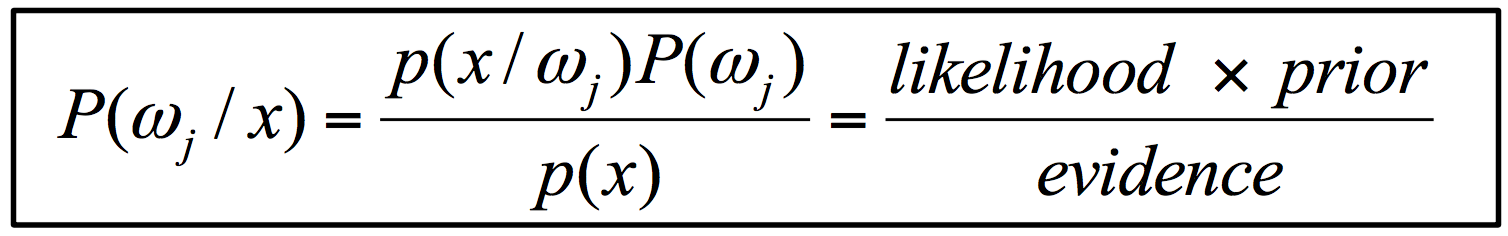
\includegraphics[scale=0.5]{Naive_bayes_general}
\end{figure}

\item Based on the instructions in the question we assume the sample distribution to be a gaussian distribution and the formula for that is as available in the question booklet. 

\begin{figure}[h!]
\centering
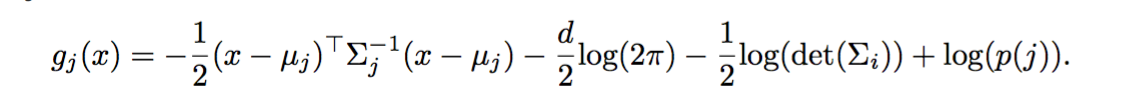
\includegraphics[scale=0.75]{MultivariateGaussian_naiveBayes}
\end{figure}

\item In this equation the $\Sigma_{i}$ is taken as the covariance of the entire data set and the $\Sigma_{j}$ is taken as the covariance matrix for that particular class for which we are computing the posterior probability.

\item This is also the discriminant function for this case. So we tag the sample to the class which gives the highest output from the discriminant function.

\item We first separate the data set into the training and testing data set with a ratio of 70\% 30\% with 140 samples for training data and 60 samples for testing data.

\item The covariance matrices, class prior and the class mean is calculated from the training data.

\item We predict the classes using the above mentioned discriminant function and plot the confusion matrix and give the error Rate. 

\item The time to give the predictions is also noted in each case.

\item the output with the error rate and the execution times are available below
\newpage
\begin{verbatim}
Calculating the Covariance Matrix for Class 0
Calculating the Covariance Matrix for Class 1
Calculating the Covariance Matrix for EntireDataSet
Elapsed time is 0.015846 seconds.

-------Testing Data -------

The Error Rate for Testing Data is 0.016667
Elapsed time is 0.912333 seconds.

----- Training Data --------

The Error Rate for Training Data is 0.007143
Elapsed time is 0.582898 seconds.

------Complete Dataset ------

The Error Rate for Complete dataset is 0.010000
Elapsed time is 0.639021 seconds.
\end{verbatim}
\item The time taken is directly proportional to the number of samples in the dataset. 
\item the figures \ref{Fig:ConfTesting}, \ref{Fig:ConfTraining} \& \ref{Fig:ConfCompleteData} are the confusion matrices obtained for the 7:3 training:testing ratio

\begin{figure}[h!]
\centering
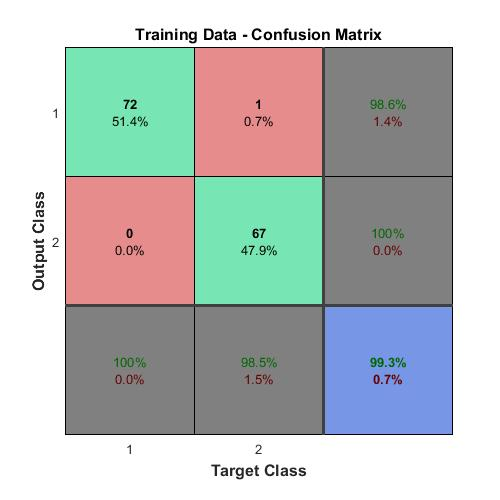
\includegraphics[scale=0.5]{TrainingData_Confusion.jpg}
\caption{Confusion Matrix for Training Data}
\label{Fig:ConfTraining}
\end{figure} 


\begin{figure}[h!]
\centering
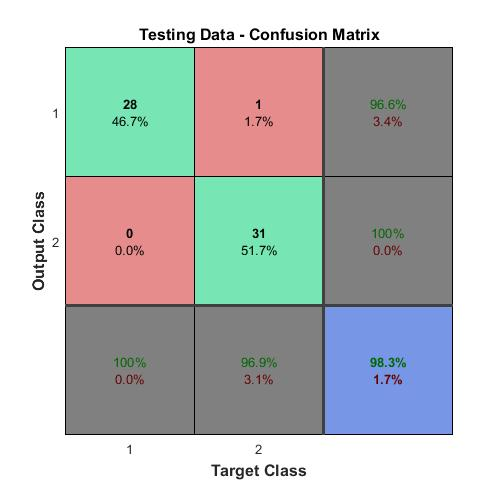
\includegraphics[scale=0.5]{TestingData_Confusion.jpg}
\caption{Confusion matrix for Testing Data}
\label{Fig:ConfTesting}
\end{figure} 


\begin{figure}[h!]
\centering
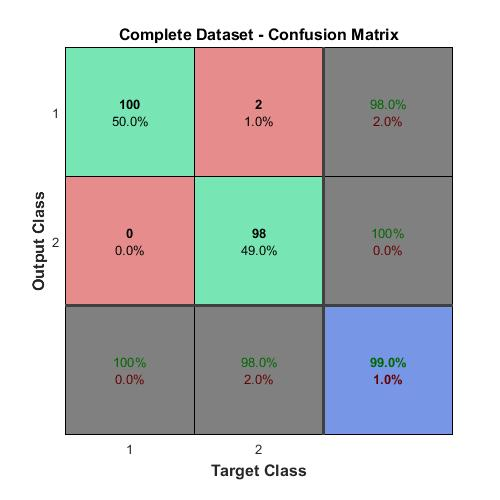
\includegraphics[scale=0.5]{CompleteDataset-Confusion-2.jpg}
\caption{Confusion Matrix for Complete Dataset}
\label{Fig:ConfCompleteData}
\end{figure} 
\end{enumerate}

\newpage
\section{}
\begin{enumerate}
\item Given the distribution to be a gaussian distribution , using the LDA approach for bayesian probability estimation we have the following formula.
\item This equation is also the discriminant function in our case. The greater than symbol explains that this is an example of Dichotomizer. Where we have 2 classes. If the $g_{1}(x) - g_{2}(x) > threshold$ we can tag the sample as class one else class two. Here $g_{i}(x)$ is discriminant function. 

\begin{figure}[h!]
\centering
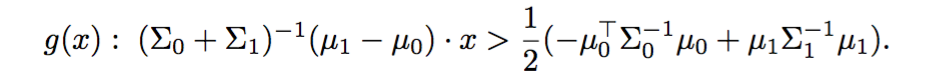
\includegraphics[scale=0.5]{LDABased}
\end{figure}
\item In our case the the threshold is assumed to be zero and the constant values in the discriminant function is moved to the right hand side to obtain the above equation 

\item the LDA based approach assumes that the class covariances are equal to achieve the equation above, where the threshold is 0. So this causes a small drop in accuracy.

\item the output with the error rate and the execution times are available below
\begin{verbatim}
Calculating the Covariance for Class 0
Calculating the covariance matrix for Class 1
Calculating the covariance matrix for EntireDataSet

Elapsed time is 0.028948 seconds.
----------- Testing Data --------------
CM =

    28     0
     2    30

The Error Rate for Testing Data is 0.033333
Elapsed time is 0.860959 seconds.

-------------Training Data ----------------
CM =

    72     0
     5    63
The Error Rate for Training Data is 0.035714
Elapsed time is 0.553176 seconds.

--------- For Complete Dataset ----------
CM =

   100     0
     7    93
The Error Rate for Complete Data is 0.035000
Elapsed time is 0.563648 seconds.

\end{verbatim}
\item The time required for the prediction is lesser than the previous set because we don't need to calculate the covariance of the entire sample dataset and the prior of the dataset.  Also the time consumption is going to be directly proportional to the number of samples in the dataset.  The LDA based approach only requires the mean and the class covariances from the training dataset. 

\item The confusion matrices for the testing training and complete dataset are available in figures \ref{Fig:ConfTraining2} \ref{Fig:ConfTesting2} \ref{Fig:ConfCompleteData2}

\begin{figure}[h!]
\centering
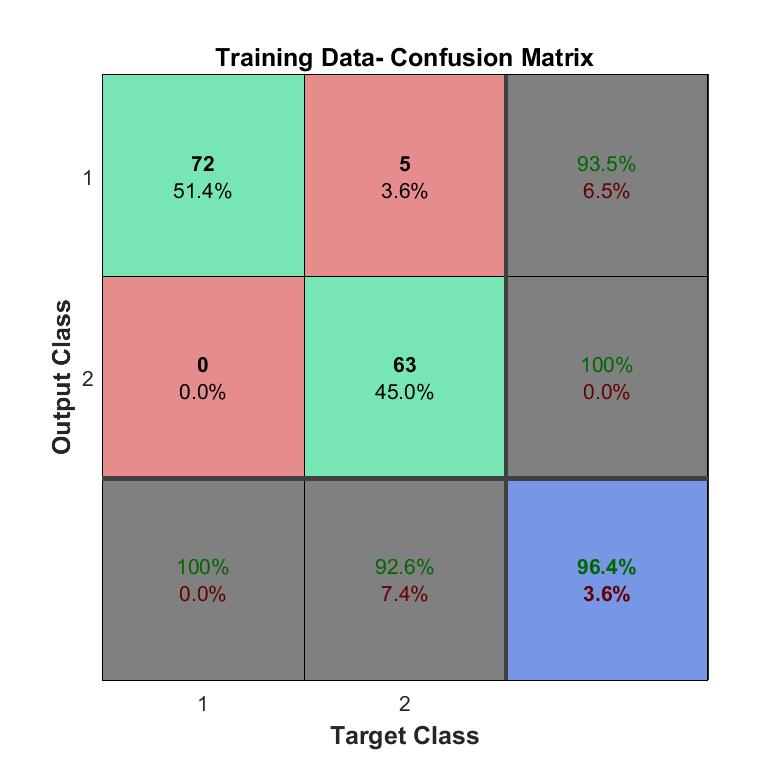
\includegraphics[scale=0.5]{TrainingData_Confusion-2.jpg}
\caption{Confusion Matrix for Training Data : Set 2}
\label{Fig:ConfTraining2}
\end{figure} 


\begin{figure}[h!]
\centering
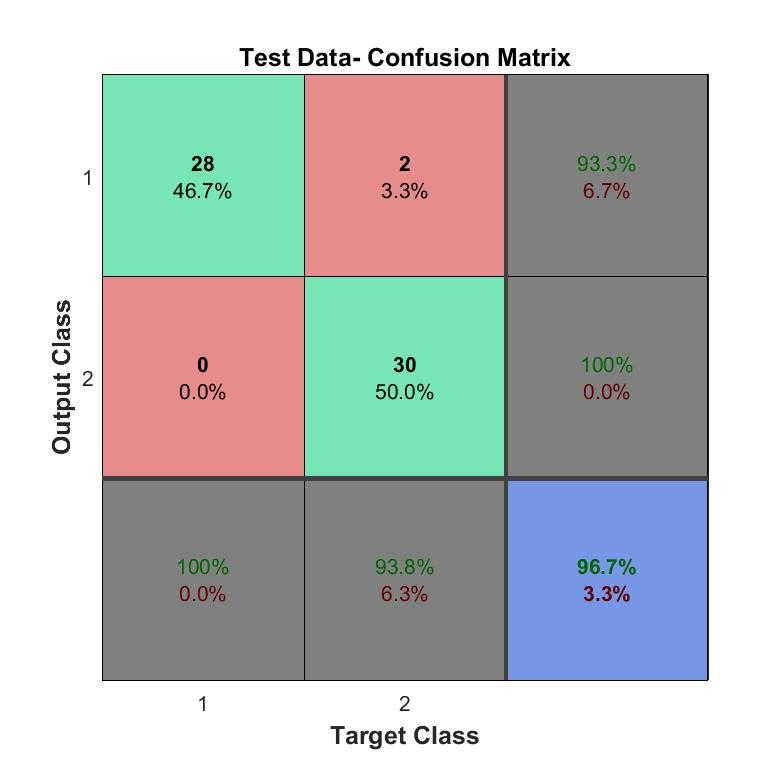
\includegraphics[scale=0.5]{TestingData_Confusion-2.jpg}
\caption{Confusion matrix for Testing Data : Set 2}
\label{Fig:ConfTesting2}
\end{figure} 


\begin{figure}[h!]
\centering
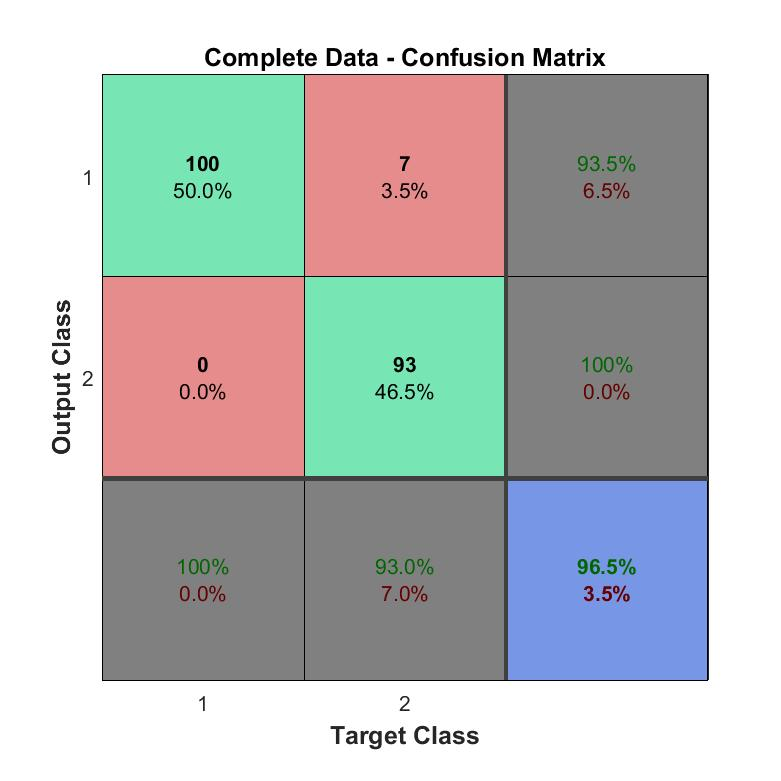
\includegraphics[scale=0.5]{CompleteDataset_Confusion-2Second.jpg}
\caption{Confusion Matrix for Complete Dataset : Set 2}
\label{Fig:ConfCompleteData2}
\end{figure} 

\item we can see that the accuracy drops for the LDA based approach because we assume that the class covariances are almost equal so that costs us in accuracy a little. In our case the accuracy drops by approximately 3\%

 \item false positives, false negatives, true positives, true negatives, accuracy and recall Explain all therse
\end{enumerate}

\section{Conclusion}

\begin{enumerate}
\item we can see that the accuracy drops for the LDA based approach because we assume that the class covariances are almost equal so that costs us in accuracy a little. In our case the accuracy drops by approximately 3\%

\item The samples which are classified into the wrong class are referred to as true negatives. 

\item The accuracy for the  normal naive bayes classifier is approximately 99\% with one to two smaples being classified worng(True Negatives). The number of True Negatives are 1,1 and 2 for class 2 for training testing and complete dataset respectively. This can be checked in the confusionmatrix.

\item The accuracy for the LDA based approach gives us approximately 96\% accuracy and the approximately two to 7 seven smaples being classified wrongly(True Negatives). The number of True Negatives are 5,2,7 for class 2 in the training, testing and the complete dataset respectively. This can also be checked in the confusion matrix.
\end{enumerate}

\end{document}